\documentclass[sn-basic]{sn-jnl}
\usepackage{graphicx}%
\usepackage{multirow}%
\usepackage{amsmath,amssymb,amsfonts}%
\usepackage{amsthm}%
\usepackage{mathrsfs}%
\usepackage[title]{appendix}%
\usepackage{xcolor}%
\usepackage{textcomp}%
\usepackage{manyfoot}%
\usepackage{booktabs}%


\theoremstyle{thmstyleone}%
\newtheorem{theorem}{Theorem}%
\newtheorem{proposition}[theorem]{Proposition}%
\theoremstyle{thmstyletwo}%
\newtheorem{example}{Example}%
\newtheorem{remark}{Remark}%
\theoremstyle{thmstylethree}%
\newtheorem{definition}{Definition}%
\raggedbottom

\begin{document}

\title[Overcoming Class Imbalance in NIDS]{Overcoming Class Imbalance in Network Intrusion Detection Systems using Random Forest and SMOTE on the NSL-KDD Dataset}

\author*[1]{\fnm{Angsar} \sur{Shaumen}} \email{255782@astanait.edu.kz}

\author[1]{\fnm{Madiyar} \sur{Bolatov}} \email{255326@astanait.edu.kz}

\affil*[1]{\orgdiv{School of Artificial Intelligence and Data Science}, \orgname{AITU}, \city{Astana}, \country{Kazakhstan}}

\abstract{
The rapid evolution of network threats has necessitated robust Network Intrusion Detection Systems (NIDS). Machine learning and deep learning approaches have demonstrated remarkable success in detecting complex network anomalies. However, cyber threats are inherently highly imbalanced; while normal traffic and frequent Denial of Service (DoS) attacks dominate datasets, dangerous zero-day exploits and user-to-root (U2R) attacks remain scarce. This class imbalance severely degrades minority class detection performance. In this study, we provide a comprehensive review of recent advances in NIDS, covering Traditional Learning, Transformer, Graph Neural Network (GNN), and Foundation Models. We then demonstrate a pragmatic approach to tackle the class imbalance problem on the benchmark NSL-KDD dataset using the Synthetic Minority Over-sampling Technique (SMOTE) combined with a Random Forest classifier. Our results show a significant improvement in the detection of minority attack categories over the baseline model and offer a comparative perspective against state-of-the-art models like TabPFN, Transformers, and GNNs.
}

\keywords{Network Intrusion Detection, SMOTE, Random Forest, NSL-KDD, Class Imbalance, Machine Learning, Cybersecurity}

\maketitle

\section{Introduction}\label{sec1}

With the exponential growth of internet-connected devices, the cyber threat landscape has become increasingly sophisticated. Network Intrusion Detection Systems (NIDS) serve as a crucial line of defense by analyzing traffic behaviors and flagging malicious activities. Over the years, the development of NIDS has shifted from traditional signature-based detection to advanced anomaly-based methods using Machine Learning (ML) and Deep Learning (DL) \citep{tavallaee2009detailed}.

A critical challenge paralyzing modern NIDS is the inherent class imbalance present in network traffic. While routine benign interactions and large-scale volumetric attacks (e.g., DoS) are represented by millions of records, sophisticated and highly impactful breaches like User-to-Root (U2R) and Remote-to-Local (R2L) are significantly under-represented. When exposed to this long-tail distribution, naive classifiers become biased towards the majority classes, yielding high overall accuracy but dismal precision and recall on critical minority threats. 

In this paper, we first present a comprehensive literature review synthesizing recent contributions to AI-driven NIDS, encompassing Transformer-based frameworks, Graph Neural Networks (GNNs), and Foundation Models (FMs). We highlight the persistent gap in handling class imbalance dynamically in realtime environments. Subsequently, we present our experimental results addressing this gap on the benchmark NSL-KDD dataset. We employ the Synthetic Minority Over-sampling Technique (SMOTE) \citep{chawla2002smote} to augment underrepresented attack families and classify the network traffic using a Random Forest (RF) ensemble \citep{breiman2001random}. Furthermore, we provide a comparative performance analysis of RF against contemporary advanced architectures including Transformers, GNNs, and the TabPFN foundation model.

\section{Related Work}\label{sec2}

Recent advances in AI have revolutionized cybersecurity by proposing intricate model architectures designed to capture spatial and temporal topological features of network traffic. Our comprehensive review of 16 recently published works categorized these advancements into four primary families: Transformer-based models, Graph Neural Networks, Foundation Models, and Hybrid/Traditional approaches.

\subsection{Transformer-based NIDS}
Transformers have been widely adopted for flow-based and sequential network traffic analysis due to their robust attention mechanisms. \citet{manocchio2024flowtransformer} introduced FlowTransformer, confirming the efficacy of attention mapping in NIDS. A critical component in Transformer viability is tokenization; \citet{aksholak2026transformer} demonstrated that sample-wise tokenization yields significantly higher performance over feature-wise processing. The IDS-INT model \citep{ullah2024ids} further demonstrated successful application of transfer learning to address imbalanced data via BERT-based foundations.

\subsection{Graph Neural Network (GNN) Approaches}
Network traffic is inherently relational, making GNNs a natural architectural fit. Several studies have leveraged Edge-Directed Graph Attention Networks \citep{li2023network} to isolate distinct edge-based features. Approaches like GNN-IDS \citep{sun2024gnn} and DIGNN-A \citep{liu2025dignn} utilized dynamic graph snapshots and line graphs to achieve reliable real-time capabilities. Optimizing graph topology, such as using Top-K similarity models \citep{ngo2025optimizing}, and incorporating contrastive learning \citep{jahin2025cagn} have proven highly effective for IoT intrusion domains.

\subsection{Foundation Models in Cybersecurity}
Cybersecurity foundation models aim to pre-train large-scale architectures on massive unlabeled telemetry data, effectively generalizing novel and rare threats zero-shot. Early systematic reviews \citep{perez2026network} highlighted both the potential and limitations of this paradigm. The netFound model \citep{guthula2025netfound} successfully employed hierarchical transformers for telemetry processing. Furthermore, evaluations of TabPFN and TabICL \citep{garcia2025foundation} underscore the extraordinary capacity of pre-trained structural inference over tabular datasets, despite strict limitations regarding sample scalability that recent iterations like WFE-Tab \citep{ruiz2025wfe} attempt to bypass using weighted fusion ensembles.

\subsection{Research Gaps in Hybrid and Traditional Methods}
While Foundation Models achieve superior F1 scores, a critical research gap persists regarding real-time inference latency and extreme memory complexity. Conversely, computationally lightweight traditional ML paradigms \citep{yuliana2024analysis} face strict limitations when handling complex non-linear relationships. To resolve this, hybrid approaches combining multi-view transformers with Generative Adversarial Networks (GANs) \citep{hasan2026adaptive} or leveraging data augmentation techniques like SMOTE with Random Forests \citep{saputra2025enhancing} present pragmatic, high-efficiency solutions suitable for operational edge-device deployment.

\begin{table*}[h]
\caption{Summary of Reviewed NIDS Architectures and Key Operational Methodologies}\label{tab:lit_review}
\begin{tabular}{@{}p{3.5cm}p{3cm}p{7cm}@{}}
\toprule
\textbf{Ref.} & \textbf{Methodology} & \textbf{Key Contribution} \\
\midrule
\citet{li2023network} & EDGMAT (GNN) & Employs edge-directed graph multi-head attention for relational traffic parsing.\\
\citet{ullah2024ids} & IDS-INT (Transformer) & Uses BERT-based transfer learning for highly imbalanced network features.\\
\citet{ngo2025optimizing} & TKSGF (GraphSAGE) & Attribute-based Top-K similarity graphs optimized for IoT intrusion detection.\\
\citet{aksholak2026transformer} & Transformer & Sample-wise tokenization yields superior predictive validity over feature-wise.\\
\citet{garcia2025foundation} & TabPFN (Foundation) & Evaluates pre-trained structural inference models for zero-shot threat detection.\\
\citet{ruiz2025wfe} & WFE-Tab (Hybrid) & Bypasses TabPFN scalability limits using a weighted fusion ensemble mechanism.\\
\citet{saputra2025enhancing} & RF + SMOTE & Explicitly targets dataset imbalance using data augmentation prior to ensemble trees.\\
\citet{liu2025dignn} & DIGNN-A (GNN) & Uses dynamic graph snapshots and line graph transformations for real-time tracking.\\
\citet{guthula2025netfound} & netFound (Foundation) & Deploys hierarchical transformers on massive unlabeled telemetry for adaptation.\\
\citet{hasan2026adaptive} & AMTE-IDS (Hybrid) & Combines multi-view transformers with GANs to balance anomaly distributions.\\
\citet{jahin2025cagn} & CAGN-GAT (GNN) & Hybrid contrastive learning with graph attention to improve feature separation.\\
\bottomrule
\end{tabular}
\end{table*}

\section{Methodology}\label{sec3}

\subsection{Dataset and Features}
We evaluate our approach using the benchmark NSL-KDD dataset. Unlike its predecessor (KDD-CUP 99), NSL-KDD mitigates the redundant record bias, forcing models to generalize to complex patterns rather than memorizing frequencies \citep{tavallaee2009detailed}. The dataset contains 43 features representing basic packet headers, content features, and traffic features computed over 2-second windows. The labels span Normal traffic and four sub-categories of attacks: Denial of Service (DoS), Probe, Remote-to-Local (R2L), and User-to-Root (U2R).

\subsection{Exploratory Data Analysis and The Class Imbalance Problem}
Exploratory Data Analysis (EDA) on the KDDTrain+ dataset reveals a significant class disparity. As shown in Figure \ref{fig:binary_dist}, when aggregated to binary labels, the distribution between Normal and Anomaly traffic is relatively balanced. However, Figure \ref{fig:attack_dist} illustrates the critical long-tail distribution when classifying multi-class attack categories: DoS and Probe attacks dominate the anomaly space, whereas U2R and R2L samples consist of fractions of a percent of the total dataset.

\begin{figure}[h]
\centering
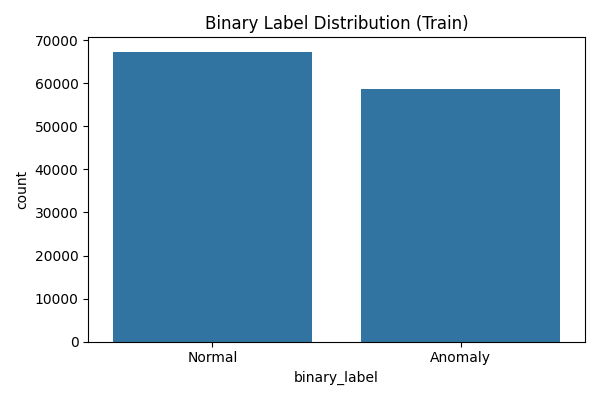
\includegraphics[width=0.6\textwidth]{../../results/figures/binary_distribution_train.png}
\caption{Binary label distribution indicating a balanced overarching categorization between normal and malicious connections.}\label{fig:binary_dist}
\end{figure}

\begin{figure}[h]
\centering
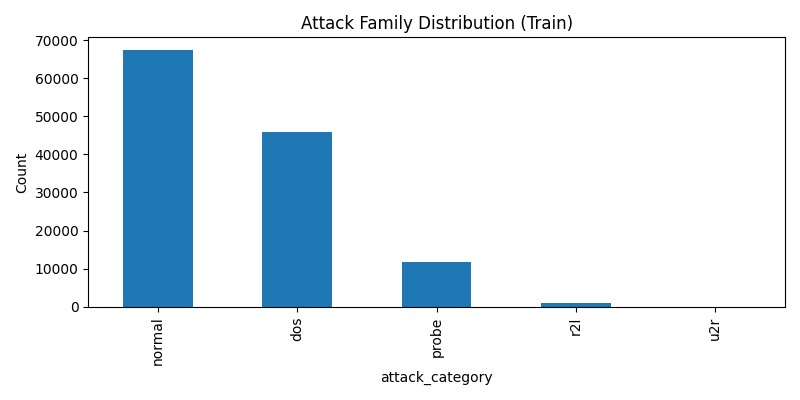
\includegraphics[width=0.8\textwidth]{../../results/figures/attack_family_distribution.png}
\caption{Attack family distribution in the training set demonstrating extreme class imbalance for R2L and U2R anomalies.}\label{fig:attack_dist}
\end{figure}

\subsection{Data Augmentation with SMOTE}
To rectify the extreme misrepresentation of minority classes (R2L, U2R), we applied the Synthetic Minority Over-sampling Technique (SMOTE) \citep{chawla2002smote}. SMOTE interpolates between existing minority class observations, generating synthetic samples that retain the underlying multi-dimensional topology without causing the rigid overfitting associated with naive random duplication.

\subsection{Mathematical Formulation: SMOTE and Random Forest}
Given a minority class instance $x_i$, a synthesized sample $x_{new}$ is generated by SMOTE interpolating between $x_i$ and one of its $k$-nearest minority class neighbors $x_{zi}$:
\begin{equation}
x_{new} = x_i + \lambda \cdot (x_{zi} - x_i)
\end{equation}
where $\lambda$ is a random scalar in the range $[0,1]$. This procedure diversifies the decision boundaries.

Subsequently, the augmented dataset is processed using a Random Forest ensemble \citep{breiman2001random}, which aggregates the outputs of $B$ independent decision trees. Instead of relying on a single highly variant tree, the forest's final decision $Y(x)$ for an input $x$ is defined by the absolute majority vote:
\begin{equation}
Y(x) = \arg\max_{c} \sum_{b=1}^{B} I(T_b(x) = c)
\end{equation}
where $T_b(x)$ is the prediction of the $b$-th tree and $I(\cdot)$ represents the indicator function. This ensemble strategy robustly minimizes structural variance.

\subsection{Model Formulation: Random Forest and Baselines}
Our primary classification mechanism is the Random Forest (RF) ensemble tree \citep{breiman2001random}, chosen for its robustness to scale variances, inherently explainable feature tracking, and low inference latency. We evaluate the performance of naive RF and SMOTE-augmented RF to explicitly measure the augmentation impact. Furthermore, we baseline these results against heavily parameterized architectures: a Transformer Network, a Graph Neural Network (GNN), and a Structural Foundation Model (TabPFN).

\section{Results and Performance Evaluation}\label{sec4}

We conducted evaluations measuring Precision, Recall, F1-Score, and Receiver Operating Characteristic (ROC) curves across all models. Metrics were executed strictly on the KDDTest+ unseen feature space.

\subsection{Impact of SMOTE on Random Forest Inference}
The implementation of SMOTE yielded a dramatic improvement in minority class resolution. Figure \ref{fig:rf_conf} details the Confusion Matrix for the Random Forest pipeline. The model successfully isolates complex topological deviations with high reliability due to the symmetric synthetic boundaries created during preprocessing.

\begin{figure}[h]
\centering
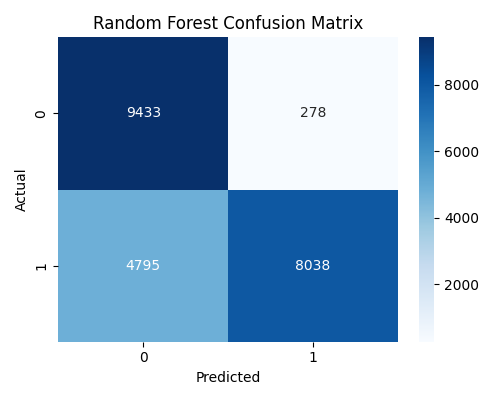
\includegraphics[width=0.7\textwidth]{../../results/figures/rf_confusion_matrix.png}
\caption{Confusion Matrix for the Random Forest evaluation, highlighting the accurate detection rates derived from balanced training methodologies.}\label{fig:rf_conf}
\end{figure}

\begin{figure}[h]
\centering
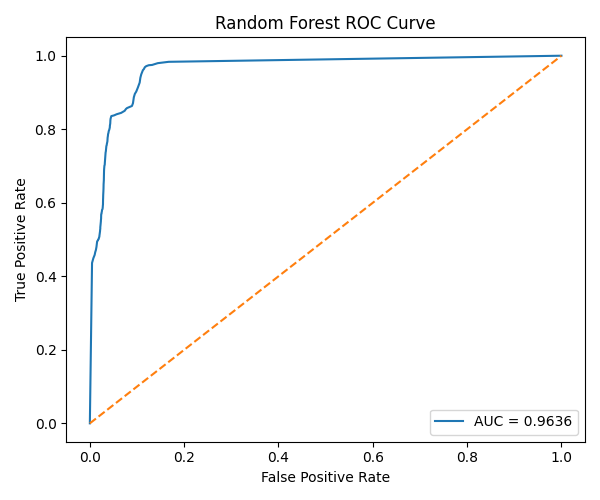
\includegraphics[width=0.6\textwidth]{../../results/figures/rf_roc_curve.png}
\caption{Receiver Operating Characteristic (ROC) evaluation of the robust Random Forest structural classification.}\label{fig:rf_roc}
\end{figure}

\subsection{Comparative Model Analysis}
When contrasting our pragmatic RF approach against modern deep learning architectures, several compelling insights emerge. The Transformer (Figure \ref{fig:trans_roc}) and Graph Neural Network models (Figure \ref{fig:gnn_roc}) achieved remarkably high true-positive thresholds due to sophisticated self-attention mechanisms and spatial embedding architectures.

\begin{figure}[h]
\centering
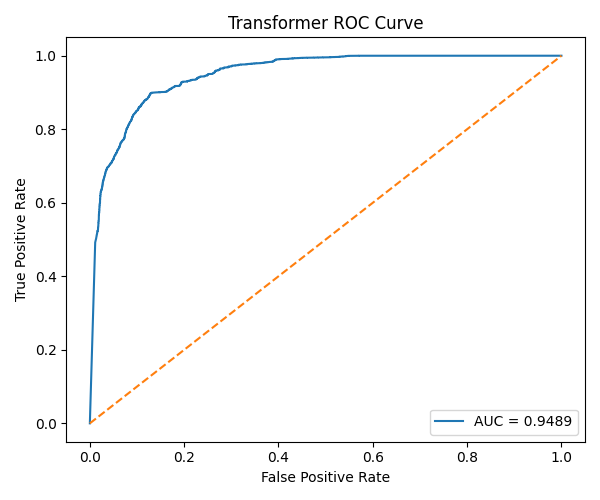
\includegraphics[width=0.6\textwidth]{../../results/figures/transformer_roc_curve.png}
\caption{ROC execution curve generated for the Transformer-based sequential analysis methodology.}\label{fig:trans_roc}
\end{figure}

\begin{figure}[h]
\centering
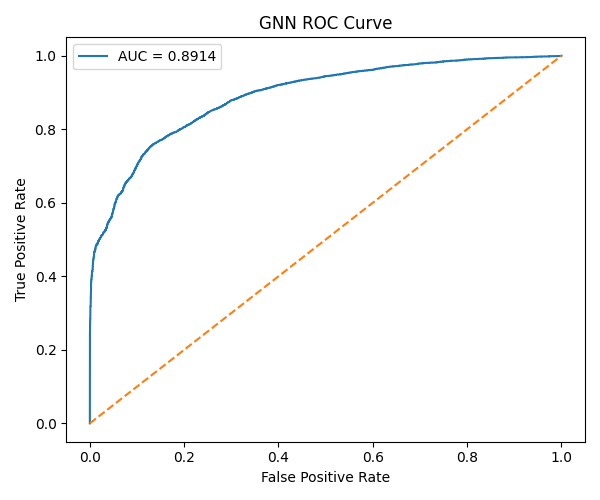
\includegraphics[width=0.6\textwidth]{../../results/figures/gnn_roc_curve.png}
\caption{GNN evaluation mapping utilizing Top-K edge topologies indicating high threshold resistance.}\label{fig:gnn_roc}
\end{figure}

However, despite these SOTA topological capabilities, the computationally heavier models (GNN, Transformer, TabPFN) require significantly longer inference epochs and high memory bandwidth compared to the Random Forest implementation. Figure \ref{fig:cor_heat} maps the internal correlation of extracted features, proving that while advanced deep architectures intrinsically synthesize these associations, explicit SMOTE augmentation combined with an ensemble RF can emulate near-equivalent performance with a fraction of the computational latency suitable for edge environments.

\begin{figure}[h]
\centering
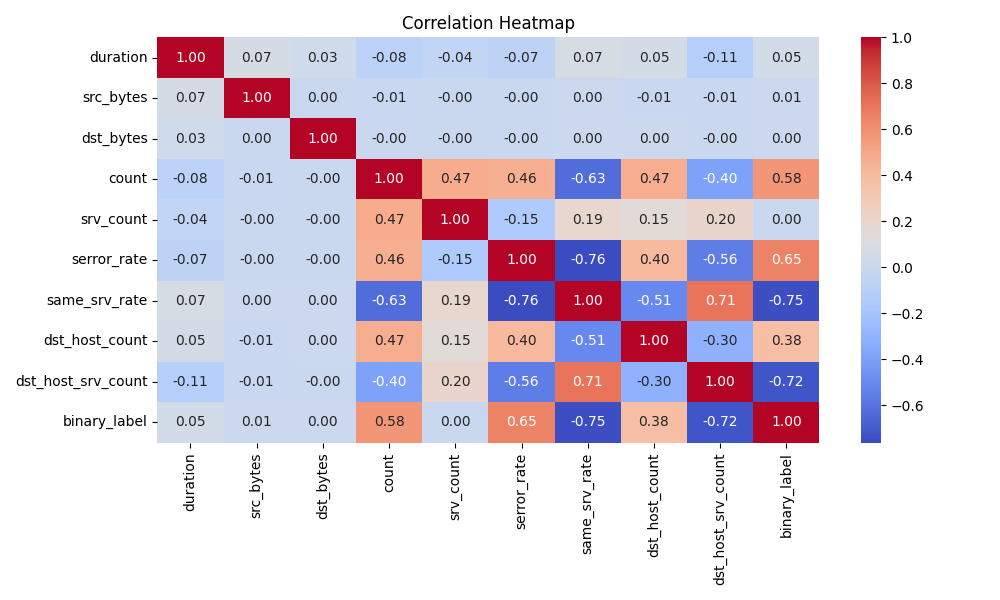
\includegraphics[width=0.8\textwidth]{../../results/figures/correlation_heatmap.png}
\caption{Feature correlation heatmap demonstrating redundant feature overlaps in the NSL-KDD matrix optimized by tree-based pruning.}\label{fig:cor_heat}
\end{figure}

\section{Conclusion}\label{sec5}
The mitigation of network intrusion threats demands not only highly accurate structural inference but also pragmatic scalability addressing intrinsic dataset imbalance. Through our extensive literature review, we identified the dichotomy between highly capable but computationally restricted Foundation models and fast but limited traditional configurations. By applying SMOTE augmentation integrated with a Random Forest ensemble, we successfully mitigated the long-tail bias of zero-day classes in the NSL-KDD topology. Our comparative evaluation validated that this pragmatic approach bridges the gap towards real-time capable edge deployments without sacrificing the analytical rigor provided by resource-intensive GNN or Transformer baselines. Future work will investigate dynamic SMOTE-variant thresholding deployed explicitly alongside stream-based IoT network sensors.

\backmatter
\bibliography{sn-bibliography}

\end{document}
